\subsection*{Variables definition}
\begin{itemize}
\item $i$= user category 
\item $j$ = promotional discount: P$_0$ = 0\%, P$_1$ = 10\%, P$_2$ = 20\%, P$_3$ = 30\%
\item $p1$ = full price of the first item (\textit{Racing skis}) 
\item $p2$ = full price of second item (\textit{Racing ski helmet})
\item $p2_j$ = price of the \textit{Racing ski helmet} when applied the promo $j$
\item $c1$ = production cost of \textit{Racing skis} = 0
\item $c2$ = production cost of \textit{Racing ski helmet} = 0
\item $q1_i(p1)$ = conversion rate for user category $i$, for \textit{Racing skis} sold at the price $p1$
\item $q2_i(p2)$ = conversion rate for user category $i$, for \textit{Racing ski helmet} sold at price the $p2$
\item $s_{ji}(p2)$ = discounted price of \textit{Racing ski helmet}, for user category $i$, according to promo discount $j$
\item $d_{ij}$ = amount of promo $j$ distributed to user category $i$
\item $d_{max}$ = maximum number of promos to be to distributed (\#P$_1$ + \#P$_2$ + \#P$_3$)
\item $avgCustomer_i$ = average number of customers for category $i$
\end{itemize}


\subsection*{Formulation of elaborated variables}
\begin{itemize}
\item $p1*q1_i(p1)*avgCustomer_i$ = revenue for the sale of \textit{Racing skis} at price $p1$ to user category $i$ 
\item $s_{ji}(p2)*q2_i(s_{ji}(p2))*d_{ij}*avgCustomer_i$  = revenue for the sale of \textit{Racing ski helmet} at the discounted price $p2$, according to the user-promo assignement 
\item $(p1*q1_i(p1)-c1*q1_i(p1))*avgCustomer_i$ = revenue for the sale of \textit{Racing skis} taking into account the production cost $c1$
\item $(q2_i(p2)*(s_{ji}(p2)*q2_i(s_{ji}(p2))*d_{ij}-q2_i(s_{ji}(p2)))*c2)*avgCustomer_i$ = revenue for the sale of \textit{Racing ski helmet} taking into account the production cost $c2$
\end{itemize}

\subsection*{Objective Function}
We have a maximization problem with the following objective function:\\
\\
$\textrm {max} ( \sum \limits _{i = 0, j = 0} ^{i = 4, j = 4}[(p1*q1_i(p1) - c1*q1_i(p1) + q2_i(p2)(s_{ji}(p2)*q2_i(s_{ji}(p2))*d_{ij} -  q2_i(s_{ji}(p2))*c2))*avgCustomer_i])$

\textbf{s.t:} $ \forall j>0 : [\sum \limits _{i = 0} ^{i = 4} d_{ij}] = d_{max} $
\\
We have fixed the full prices of the two items: $p1$, $p2$. We retrieve the discounted prices of $p2$, applying the promos $j$. \\
We know: the average number of customers per category $i$, $avgCustomer_i$, the conversion rate for both products ($q1_i(p1)$, $q2_i(p2)$) and the maximum number of promos to distribute ($d_{max}$).\\
As assumption the production costs of the two items is zero ($c1$ = 0, $c2$ = 0).\\
It is possible to retrieve the total revenue for \textit{Racing skis} as the product between the full price of the first item, the conversion rate for the considered user category and the average number of customers for that category:
$(p1 * q1_i(p1) * avgCustomer_i)$.\\
For the second item the calculation of the reward is the same except for the fact that the product is buyed only if also the first one is purchased (so we multiply also the conversion rate of the first item) and the considered price have to be discounted according to the assigned promotion. 

The solution of our optimization problem consists in the distribution of the fraction of promo codes among the user categories.

\subsection*{Offline problem - designed algorithm}

In this scenario we have to find the optimal solution in an offline manner (a solution to our maximization problem knowing all the parameters), considering the constraints that the shop uses a randomized approach to assure that a fraction of the customers of a given category gets a specified promotion according to the optimal solution.\\
We achieve the solution of the problem using a matching approach. 
To reach the optimal solution we have used an iterative approach: we build a matrix category-promotion containing the mean expected rewards for every couple, calculated as the conversion rate of the \textit{Racing ski helmet} multiplied with its discounted price.
The goal is to obtain, for each category-promotion couple the fraction of customers that will receive this discount.\\
We exploit this matrix to perform the matching between the customer classes and the promo types, in order to maximize the total reward. \\
We select the best reward for every class, for four times, retrieving, at every iteration, the four best combination of category-promotion and assigning an infinite weight to the obtained sub-optimal matching.\\
Every matching is represented by a reward configuration that maximize the total reward. Every iteration is weighted and represent a different goodnesses of the solution, the first is the best, the last is the worst.\\
Through the sub-optimal matchings, we have retrieved the fractions of different promos to assign to every customer categories, based on the proportional weight of the previous sub-optimal matching.\\
The proportions retrieved, are normalized category per category.

PESEUDOCODICE
\begin{center}
	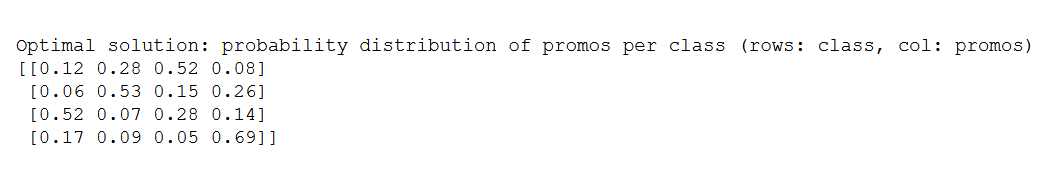
\includegraphics[scale=0.9]{Images/n1_results}
\end{center}
\begin{center}
	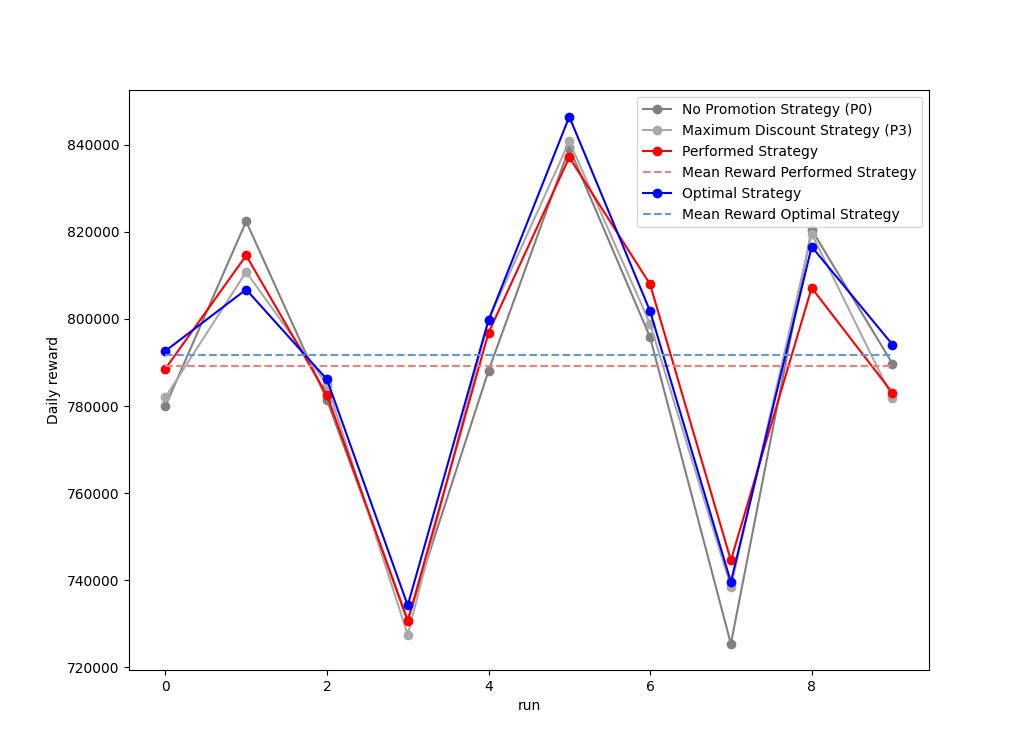
\includegraphics[scale=0.7]{Images/n1_chart}
\end{center}





